En esta etapa, se lleva a cabo la implementación del diseño del proceso ETL previamente definido, utilizando las herramientas seleccionadas. Se desarrollan los flujos de extracción, transformación y carga de los datos según lo establecido en el diseño.

Una vez implementado, se procede a realizar pruebas exhaustivas para garantizar el correcto funcionamiento del proceso. Estas pruebas incluyen la verificación de la extracción de datos de las fuentes, la correcta aplicación de las transformaciones definidas y la carga exitosa de los datos en el destino final.

El objetivo de las pruebas es asegurar que el proceso ETL cumpla con los requisitos establecidos y que los resultados obtenidos sean los esperados. Esto implica validar la integridad y coherencia de los datos transformados, así como verificar el rendimiento y la escalabilidad del proceso.

En caso de encontrar inconvenientes o desviaciones durante las pruebas, se realizan los ajustes necesarios en el diseño o en la configuración de las herramientas utilizadas. Es fundamental realizar iteraciones y pruebas adicionales hasta obtener resultados consistentes y satisfactorios.

Como primer paso en la construcción del proceso ETL, se importan las bibliotecas pandas, numpy y date proveniente de la biblioteca integrada datetime. Luego se establece la mes para ser usado como parametro de fecha y se realiza una lectura de los datos creando un dataframe de pandas para poder ser visualizados y procesados.

Como segundo paso se establecío el formato de fecha 'YYYY;MM;DD;HH;MM;SS.ss' para la columna 'fecha evento' y se eliminaron del dataframe todas las filas que contenian valores nulos.


\begin{figure}[H]
    \begin{minipage}[t]{0.8\textwidth}
        \caption{Construcción proceso ETL con Python.}
        \label{construccETL}        
    \end{minipage}

    \vspace{10pt}

    \begin{minipage}[b]{1.1\textwidth}
        \centering
        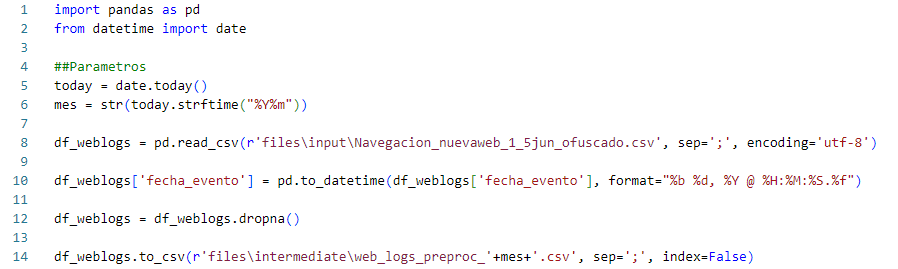
\includegraphics[width=\textwidth]{img/etl-white-ide.png}        
    \end{minipage}

    \begin{minipage}[t]{0.9\textwidth}
        Fuente: Elaboración propia.
    \end{minipage}
\end{figure}

Para finalizar el proceso ETL se guarda el dataframe procesado en un archivo .csv dentro de los archivos del proyecto.